%%%%%%%%%%%%%%%%%%%%%%%%%%%%%%%%%%%%%%%%%%%%%%%%%%%%
%%%  iScience (Cell Press) version
%%%  Build:  latexmk -pdf publication-iscience.tex
%%%%%%%%%%%%%%%%%%%%%%%%%%%%%%%%%%%%%%%%%%%%%%%%%%%%

\PassOptionsToPackage{left}{lineno}   % must precede authblk
\documentclass[12pt,letterpaper]{article}
\usepackage[a4paper, total={7in, 10in}]{geometry}
\renewcommand{\familydefault}{\sfdefault}
\usepackage{helvet}
\usepackage{authblk}
\usepackage{hyperref}

\usepackage[nohyperlinks]{acronym}
\newcommand{\loadacronyms}{\input{acronyms}}
\usepackage{graphicx}
\usepackage{booktabs}
\usepackage{tabularx}
\usepackage{amsmath}
\usepackage{fvextra}          % shared sections use \begin{Verbatim}
\usepackage{float}
\usepackage{caption}
\captionsetup[table]{justification=raggedright,singlelinecheck=false}
\captionsetup[figure]{justification=raggedright,singlelinecheck=false}

\usepackage{lineno}
\linenumbers

%%% ── Compatibility shims for shared section files ──
%%% Section files use numbered \section{}; render unnumbered:
\setcounter{secnumdepth}{0}

%%% Section files use figure*/table*; map them to single-column figure/table:
\renewenvironment{figure*}{\begin{figure}}{\end{figure}}
\renewenvironment{table*}{\begin{table}}{\end{table}}

\makeatletter
\renewcommand{\maketitle}{\bgroup\setlength{\parindent}{0pt}
\begin{flushleft}
  \textbf{\@title}
  
  \@author
\end{flushleft}\egroup}
\makeatother

%%%  Title

\title{A systematic evaluation and benchmarking of text summarization methods for biomedical literature: From word-frequency methods to language models}

%%%  Authors and affiliations

\author[1,4]{Fabio Baumgärtel}
\author[1,2,4]{Enrico Bono}
\author[1]{Lucas Fillinger}
\author[1,2]{Louiza Galou}
\author[1]{Kinga Keska-Izworska}
\author[1]{Samuel M Walter}
\author[1]{Peter Andorfer}
\author[1,2]{Klaus Kratochwill}
\author[1,3]{Paul Perco}
\author[1,2,5,*]{Matthias Ley}

\affil[1]{Delta4 GmbH, Vienna, Austria}
\affil[2]{Division of Pediatric Nephrology and Gastroenterology, Department of Pediatrics and Adolescent Medicine, Comprehensive Center for Pediatrics, Medical University Vienna, Vienna, Austria}
\affil[3]{Department of Internal Medicine IV, Medical University Innsbruck, Innsbruck, Austria}
\affil[4]{These authors contributed equally}
\affil[5]{Lead contact}
\affil[*]{matthias.ley@delta4.ai}

%%%  Bibliography — Numbered (AMA) style
\usepackage[super,comma,sort&compress]{natbib}\bibliographystyle{numbered}


\begin{document}

\maketitle

\loadacronyms

\section*{Summary}

The rapid expansion of biomedical literature demands automated summarization tools that reliably condense research articles into concise, accurate summaries. We benchmarked 62 summarization methods, ranging from frequency-based and TextRank extractors to encoder-decoder models (EDMs) and large language models (LLMs), on 1,000 biomedical abstracts from 20 journals across \textit{ScienceDirect} and \textit{Cell Press}, using author-written highlights as reference summaries. Models were evaluated with a composite suite of lexical, semantic, and factual metrics, including ROUGE, BLEU, METEOR, embedding-based similarity, and factuality scores. General-purpose models (e.g., Mistral, GPT, Llama) achieved the highest overall performance across lexical and semantic dimensions, outperforming reasoning-oriented (e.g., DeepSeek, Magistral) and domain-specific (e.g., BioGPT, BioMistral) models. Notably, medium-sized models outperformed large-scale models, suggesting an optimal balance between model capacity and efficiency, while classical extractive methods lagged behind neural approaches. These findings provide a systematic reference for selecting biomedical summarization tools and highlight that broad pretraining outperforms narrow domain adaptation.

\section*{Keywords}

biomedical text summarization, natural language processing, large language models, benchmarking

%%% ── Shared sections (with their own \section{} headers) ──

\section{Introduction}

The exponential growth of scientific literature has created a demand for text summarization methods to support scientists in prioritizing articles, extracting relevant information, and interpreting research findings. \ac{ATS} methods have evolved from statistical approaches to deep learning-based models, thus becoming increasingly sophisticated and reliable in capturing the essential parts of complex research articles. Although \ac{ATS} methods have been previously evaluated and described  \cite{zhang2025comprehensivesurveyprocessorientedautomatic,zhang2024systematicsurveytextsummarization}, only a few have focused on scientific literature \cite{ROHIL2022100058,xie2023surveybiomedicaltextsummarization}. Recent work has begun to benchmark \acp{LLM} on biomedical summarization, though only for a limited set of models and typically against abstract-based references \cite{chen2025benchmarking,celikten2025benchmarking,toprak2025benchmarking}. A systematic comparison from word-frequency methods to state-of-the-art \acp{LLM} is still lacking.

Over time, these methods have developed into distinct approaches that differ in how they identify or generate summary content. Early pre-neural summarization was mainly characterized by unsupervised extractive approaches that rank sentences by word or concept frequencies to identify relevant sentences. The field was initially shaped by Luhn's assumption that recurrent words signal importance   \cite{Luhn1958TheAC} and Edmundson's use of cue words, title words, and sentence position \cite{10.1145/321510.321519}. Later work adopting weighting \ac{TF-IDF} refined this idea by down-weighting frequent, low-specificity terms \cite{article}, laying the foundation for more advanced methods in scientific text summarization \cite{10.1145/1183614.1183701}. Graph-based methods judged the importance against the document's global structure rather than local word counts. TextRank, widely used in the biomedical domain, applies the PageRank algorithm to a sentence-similarity graph to select top-ranked sentences \cite{mihalcea-tarau-2004-textrank}. 

The advent of \ac{Seq2seq} frameworks shifted the field toward neural approaches capable of paraphrasing and condensing text using encoder-decoder architectures, originally implemented with \acp{RNN}, \ac{LSTM} networks, and \acp{GRU} \cite{afzal2020, almasoud2022}, while self-attention enabled parallel processing of sequences and modeling of long-range context  \cite{vaswani2023attentionneed}. This laid the foundation for transformer architectures that quickly gained popularity in performing a wide range of \ac{NLP} tasks. Building on \ac{BERT} \cite{devlin2019bertpretrainingdeepbidirectional}, several abstractive summarization models have emerged, including \ac{BART}, a denoising autoencoder for pretraining \ac{Seq2seq} models \cite{DBLP:journals/corr/abs-1910-13461} and its biomedical adaptations \cite{yuan-etal-2022-biobart, abinaya2024}; the unified \ac{T5} model \cite{JMLR:v21:20-074}; \ac{PEGASUS} \cite{zhang2020pegasuspretrainingextractedgapsentences}, including domain-specific PubMed variants; and Longformer-based models \cite{Beltagy2020Longformer} that can handle longer inputs \cite{steblianko2024}. These models are typically pretrained independently, while Longformer-based variants may additionally leverage \ac{RoBERTa}, an optimized version of \ac{BERT} trained on a larger corpus.   

More recently, the field of \ac{ATS} has quickly moved toward decoder-only architectures at the core of \acp{LLM}, which capture semantic relations with greater flexibility and specificity. \acp{LLM} can be classified as (i) general-purpose models, which apply broad domain knowledge across diverse \ac{NLP} tasks, such as the proprietary \ac{GPT} \cite{Radford2018ImprovingLU} and Claude \cite{bai2022constitutionalaiharmlessnessai} series and the open-source \ac{Llama} \cite{grattafiori2024llama3herdmodels} and Gemma \cite{gemmateam2025gemma3technicalreport} families; (ii) reasoning-oriented models, characterized by logical text understanding through iterative chain-of-thought processing and instruction tuning \cite{plaat2025multistepreasoninglargelanguage} such as DeepSeek-R1 \cite{wang2025reviewdeepseekmodelskey}, Qwen3 \cite{qwen3technicalreport}, and Mistral's Magistral \cite{mistralai2025magistral}, together with the reasoning tiers of the proprietary families (e.g., GPT-5 and Claude Opus 4); and (iii) domain-specific models, tailored for specialized tasks or specific scientific domains , such as the biomedical models OpenBioLLM-Llama3 \cite{OpenBioLLMs}, BioGPT \cite{10.1093/bib/bbac409}, and BioMistral \cite{labrak2024biomistral}, and SciLitLLM \cite{li2025scilitllmadaptllmsscientific} for scientific literature. The gold-standard dataset used for benchmarking and the complete set of models evaluated in this study are listed in Tables~\ref{tab:goldstandard} and \ref{tab:models} in the STAR Methods section.

Despite this range of approaches, these method families have not been evaluated together on biomedical literature, leaving little guidance on which to choose. This study addresses this gap by systematically evaluating 62 text summarization models, ranging from word-frequency methods to state-of-the-art \acp{LLM}, using a dataset of 1,000 biomedical abstracts and corresponding highlights sections as reference summaries. We provide recommendations for selecting appropriate tools to accelerate knowledge discovery in biomedical sciences and discuss the strengths and limitations of each approach.  

\input{Sections/materials_methods}

\section{Results}

Our benchmark results offer a comparative view of summarization performance across all evaluated models. We first examined the correlations among the chosen evaluation metrics and, based on the findings, identified the best-performing model across lexical, semantic, and factual dimensions. Next, we compared model performance across categories and families to identify significant differences. We additionally performed a data leakage analysis to ensure that inclusion of benchmarking data in training data had no impact on the results. We then analyzed how well automatic metrics aligned with human judgment based on expert level result assessment, and finally assessed whether an \ac{LLM}-as-a-judge panel could reproduce these rankings.

\subsection{Metric Correlations}

Pairwise Spearman correlations were computed to analyze the relationships between the different evaluation metrics (Figure~\ref{fig:metric_correlation}). Strong positive correlations were observed among most lexical-based metrics (\ac{ROUGE}-1/2/L, \ac{METEOR}, and \ac{BLEU}), with the correlation between \ac{METEOR} and \ac{BLEU} marking an exception ($\rho = 0.23$). \ac{ROUGE} variants showed almost identical behavior ($\rho \geq 0.88$), while \ac{BLEU} and \ac{METEOR} demonstrated slightly weaker but still substantial alignment with \ac{ROUGE} measures ($\rho = 0.51 - 0.82$).

Most semantic-based metrics (\ac{RoBERTa}, \ac{DeBERTa}, and all-mpnet-base-v2) showed high internal consistency ($\rho > 0.5$), reflecting their shared focus on semantic similarity. When compared with lexical-based metrics, correlations were moderate to strong in most cases, indicating that both categories capture related but not identical dimensions of summary quality. 

Concerning factual consistency metrics, AlignScore and the two MiniCheck variants exhibited very strong correlations with each other ($\rho = 0.82 - 0.94$), while SummaC showed moderately positive correlations with the other factual metrics ($\rho = 0.41 -0.69$). This likely reflects methodological differences, as SummaC relies on zero-shot natural language inference over sentence pairs, while MiniCheck and AlignScore use models specifically optimized for factual consistency assessment. When compared with lexical- and semantic-based metrics, correlations were generally weaker and, in some cases, even slightly negative. This pattern can largely be attributed to the different point of reference used by factual metrics.

Overall, these relationships demonstrate that the various metrics are broadly consistent while providing complementary perspectives. This supports the use of an aggregated ``Overall Performance Score'' as a balanced indicator of overall summarization performance.

\subsection{Overall Model Performance}

Based on overall performance ranks, referred to as ``Performance Rank" and derived from our multi-metric evaluation framework (\ref{subsec:overall_performance_metric} Overall Performance Metric), models from the Mistral family were top-ranked across the three evaluated metric dimensions, as depicted in Figure~\ref{fig:rank_heatmap}. 

The mistral-small3.2:24b model ranked first, followed by mistral-small-2506 and mistral-medium-2505. The lowest-ranked models included OpenBioLLM-Llama3-8B, bigbird-pegasus-large-pubmed and pegasus-pubmed from the \ac{PEGASUS} family, and mT5\_multilingual\_XLSum from the \ac{T5} family. Overall, domain-specific \acp{SLM} and \ac{EDM} models showed poor performance across all the different dimensions of metrics.

Among the ten top-ranked models, six were general-purpose \acp{LLM} and four were general-purpose \acp{SLM}. A similar trend was observed in the top half of the ranking (positions 1 to 31) with the presence of just a few reasoning-oriented and domain-specific models. In contrast, in the lower half of the ranking, where models performed poorly across most metric dimensions, the majority were reasoning-oriented \acp{SLM}, general-purpose \acp{EDM}, domain-specific \acp{EDM}, and traditional models. 

Considering each metric dimension separately, several Mistral models ranked high in the lexical dimension, with GPT-5-nano, a reasoning-oriented \ac{LLM} from the \ac{GPT} family, ranking third. In the semantic dimension, Mistral models achieved high ranks, but the highest positions were occupied by the Phi4:14b general-purpose \ac{LLM} and several Granite models, including granite4:tiny-h and granite3.3:2b. Finally, the highest ranks based on the factual dimension were covered by traditional models and some \acp{EDM}. Detailed performance indications for each model across all individual ranked metrics are provided in Supplementary Figure~\ref{fig:supplementary_overview}.

Models could also decline to summarize by returning the INSUFFICIENT\_FINDINGS token. This was rare overall, occurring in 736 of 62,000 generated summaries (1.2\%) and exclusively among prompt-based models. Usage was concentrated in the two domain-specific biomedical models OpenBioLLM-Llama3-8B (20.0\%) and medllama2 (9.7\%), while all other models returned it in fewer than 6\% of cases.

\subsection{Category Comparisons}

To compare model performance across categories, we displayed the distribution of overall performance scores within each category, along with the best- and worst-performing individual models (Figure~\ref{fig:category_boxplots_and_gameshowell}a). Results of the Games-Howell post-hoc comparisons between individual groups are given in Figure~\ref{fig:category_boxplots_and_gameshowell}b.

All general-purpose \acp{LLM} achieved high overall scores, thus forming the top category of models, with general-purpose \acp{SLM} following second, however showing a slightly wider spread in performance scores. Domain-specific \acp{LLM} and reasoning-oriented \acp{LLM} followed in third and fourth place based on average overall performance.

Domain-specific \acp{EDM}, domain-specific \acp{SLM}, traditional models, and general-purpose \acp{EDM} performed significantly worse as compared to general-purpose \acp{LM}. Domain-specific \acp{EDM} and domain-specific \acp{SLM} displayed the widest spread of performance (Figure~\ref{fig:category_boxplots_and_gameshowell}a).

\subsection{Family Comparisons}

To complement the category-level findings, we examined performance across model families, since models within the same family often share architectural features or training strategies that may cause consistent performance trends. Figure~\ref{fig:family_boxplots_and_gameshowell}a shows the distribution of overall performance scores across all model families. Similar to the category-level analysis, there were clear performance differences between architectural lineages. The Mistral family achieved the strongest overall results, with several members ranking among the top performers in the benchmark. Families dominated by modern \ac{LLM} or \ac{SLM} architectures, such as Granite, Claude, and Gemma, consistently outperformed more traditional extractive approaches and families built on encoder-decoder architectures such as \ac{LED}, \ac{BART}, \ac{T5} and \ac{PEGASUS}.

In particular, the \ac{GPT} and \ac{Llama} families showed lower performance scores than expected given the competitive performance of their top models. This was primarily due to the inclusion of domain-specific small models, such as BioGPT and OpenBioLLM-Llama3-8B, which performed substantially worse than their general-purpose counterparts and therefore pulled down the family-level averages.

Regarding the Games-Howell post-hoc matrix in the family comparison (Figure~\ref{fig:family_boxplots_and_gameshowell}b), a combination of significant and non-significant differences between families was observed, reflecting the greater heterogeneity within some lineages. While many high-performing families differed significantly from traditional and encoder-decoder dominated families, several comparisons among modern \acp{SLM} and \acp{LLM} dominated families did not reach statistical significance.

\subsection{Data Leakage Assessment}

\subsubsection{Cutoff Overlap Results}

Across the evaluated models, potential overlap ranged from minimal levels of 5\% for earlier models with training cutoffs prior to 2024, up to 40.2\% for more recent \acp{LLM} with reported cutoff dates in early 2025. Most models showed low overlap ($\leq 20\%$), indicating that the majority of benchmark articles were published after their respective training cutoff dates. A subset of eight models, including recent versions of Claude, Deepseek, and one \ac{GPT} model, exhibited moderate levels of potential overlap ($24 - 40.2\%$) and were further analyzed via an abstract completion probe in the next step.

A complete overview of training cutoff dates and corresponding potential overlap values for all models is provided in Supplementary Table~\ref{tab:training_cutoff_overlap}.

\subsubsection{Abstract Completion Probe}

To assess whether high potential overlap translated into memorization effects, we conducted an abstract completion probe for the eight models showing moderate levels of potential overlap. For each model \ac{ROUGE}-L scores between generated completions and the original abstracts were compared for articles published before and after the respective training cutoff dates.

Average \ac{ROUGE}-L scores were nearly identical for pre-cutoff and post-cutoff articles (both at approximately 13.5\%) and there were only negligible differences at the individual model level (Table~\ref{tab:completion_probe}). Statistical testing using a one-sided Mann-Whitney U test revealed no significant increase in similarity for pre-cutoff articles in any of the tested models. Effect sizes were consistently close to zero, which further indicates that there is no systematic difference between the two groups.

If memorization effects had occurred, substantially higher similarity scores would be expected for abstracts from pre-cutoff articles. As this was not the case, we concluded that the models were not reproducing memorized content from their training data.

\subsection{Expert Assessment Results}

The results of the expert assessment are summarized in Figure~\ref{fig:assessment_results} and Table~\ref{tab:human_eval}. Values are reported as mean $\pm$ \ac{SEM}. The two Mistral-based models (mistral-small3.2:24b and mistral-small-2506) consistently outperformed the two \acp{EDM} (bigbird-pegasus-large-pubmed and mT5\_multilingual\_XLSum) across all four evaluation dimensions.

For coherence and fluency, both Mistral models scored substantially higher than the \acp{EDM}. In coherence, they reached scores of 4.83 $\pm$ 0.03 and 4.82 $\pm$ 0.04, compared with 3.20 $\pm$ 0.10 for mT5 and 2.08 $\pm$ 0.08 for bigbird-pegasus. The same pattern was observed for fluency, where the Mistral models achieved scores of 4.86 $\pm$ 0.03 and 4.90 $\pm$ 0.03, clearly exceeding mT5 (3.67 $\pm$ 0.09) and bigbird-pegasus (2.23 $\pm$ 0.07). All pairwise comparisons between Mistral models and \acp{EDM} were statistically significant (all $p < 0.001$ after Bonferroni correction). The two \acp{EDM} also differed significantly from each other in both dimensions, while no significant differences were found between the two Mistral models.

Differences were even more pronounced for relevance and consistency. The Mistral models again achieved high scores in relevance (4.07 $\pm$ 0.07 and 4.09 $\pm$ 0.07), while mT5 (1.54 $\pm$ 0.06) and bigbird-pegasus (1.40 $\pm$ 0.05) scored markedly lower. A similar pattern was seen for consistency, where the Mistral models reached scores of 4.56 $\pm$ 0.06 and 4.59 $\pm$ 0.05, compared to 2.17 $\pm$ 0.09 for mT5 and 1.41 $\pm$ 0.05 for bigbird-pegasus. Again, all Mistral versus \ac{EDM} comparisons were statistically significant ($p < 0.001$). The \acp{EDM} differed significantly in consistency, but not in relevance ($p = 0.7308$), and no significant differences were found between the two Mistral models.

Inter-rater agreement was strong on both measures. Gwet's AC2 indicated substantial absolute agreement across all dimensions, ranging from 0.713 (relevance) to 0.794 (fluency), with an overall value of AC2 = 0.725. Mean pairwise Spearman correlations were likewise strong across all dimensions, ranging from $\rho = 0.707$ (coherence) to $\rho = 0.801$ (consistency), with an overall mean of $\rho = 0.765$ (all $p < 0.001$). These results show that evaluators consistently agreed both on the absolute quality of the summaries and on the relative ranking between models.

\subsection{LLM-as-a-Judge Evaluation}
The LLM-as-a-judge panel agreed closely with expert assessments on every dimension (Table~\ref{tab:judge-expert}). To benchmark against human reliability, we computed a leave-one-out ceiling on the same target the judges were scored against: each expert's ratings were correlated against the mean of the remaining experts. The judge's mean agreement ($\rho=0.87$) exceeded this ceiling ($\rho=0.82$), leading to the assumption that it tracked the expert consensus at least as closely as a typical individual expert.


The judge panel did not separate the four dimensions well. Its agreement with the matching expert dimension (diagonal $\rho=0.87$) was barely higher than its agreement with the other dimensions (off-diagonal $\rho=0.85$), a gap of only $0.02$. In effect the judge measured a single overall-quality signal rather than four independent constructs, so its per-dimension scores should not be over-interpreted.

We questioned whether the LLM-as-a-judge panel was capable of ranking the 62 models in a comparable manner to the evaluation metrics (Table~\ref{tab:concordance}). The judge ranking agreed strongly with the lexical, semantic, and composite performance ranks ($\rho=0.75$-$0.83$). The factual metrics were an exception ($\rho=0.09$, n.s.), as they reward verbatim copying, so extractive systems (TextRank, frequency, T5, PEGASUS) ranked highly on factuality but performed poorly under the judge - a construct difference rather than a judge failure.

To analyze the tendency of judges to favor their own model family, we computed, for each judge, how far its score sat above or below the mean of the other two judges, and contrasted its own-family models with all others (Table~\ref{tab:selfpref}). Anthropic exhibited a clear self-preference effect ($+0.30$ on the 1-5 scale), whereas OpenAI and Mistral showed no detectable differential effect ($\leq 0.08$ in magnitude). The direction is consistent with self-preference reported for rubric-based judging \citep{panicksseryLLMEvaluatorsRecognize2024,pombalSelfPreferenceBiasRubricBased2026}. Taking the median across the three judges damped this bias in the final scores.



\input{Sections/discussion}

\input{Sections/conclusions}

%%% ── Back matter ──

\section*{Supplemental information}

\begin{figure}[H]
    \centering
    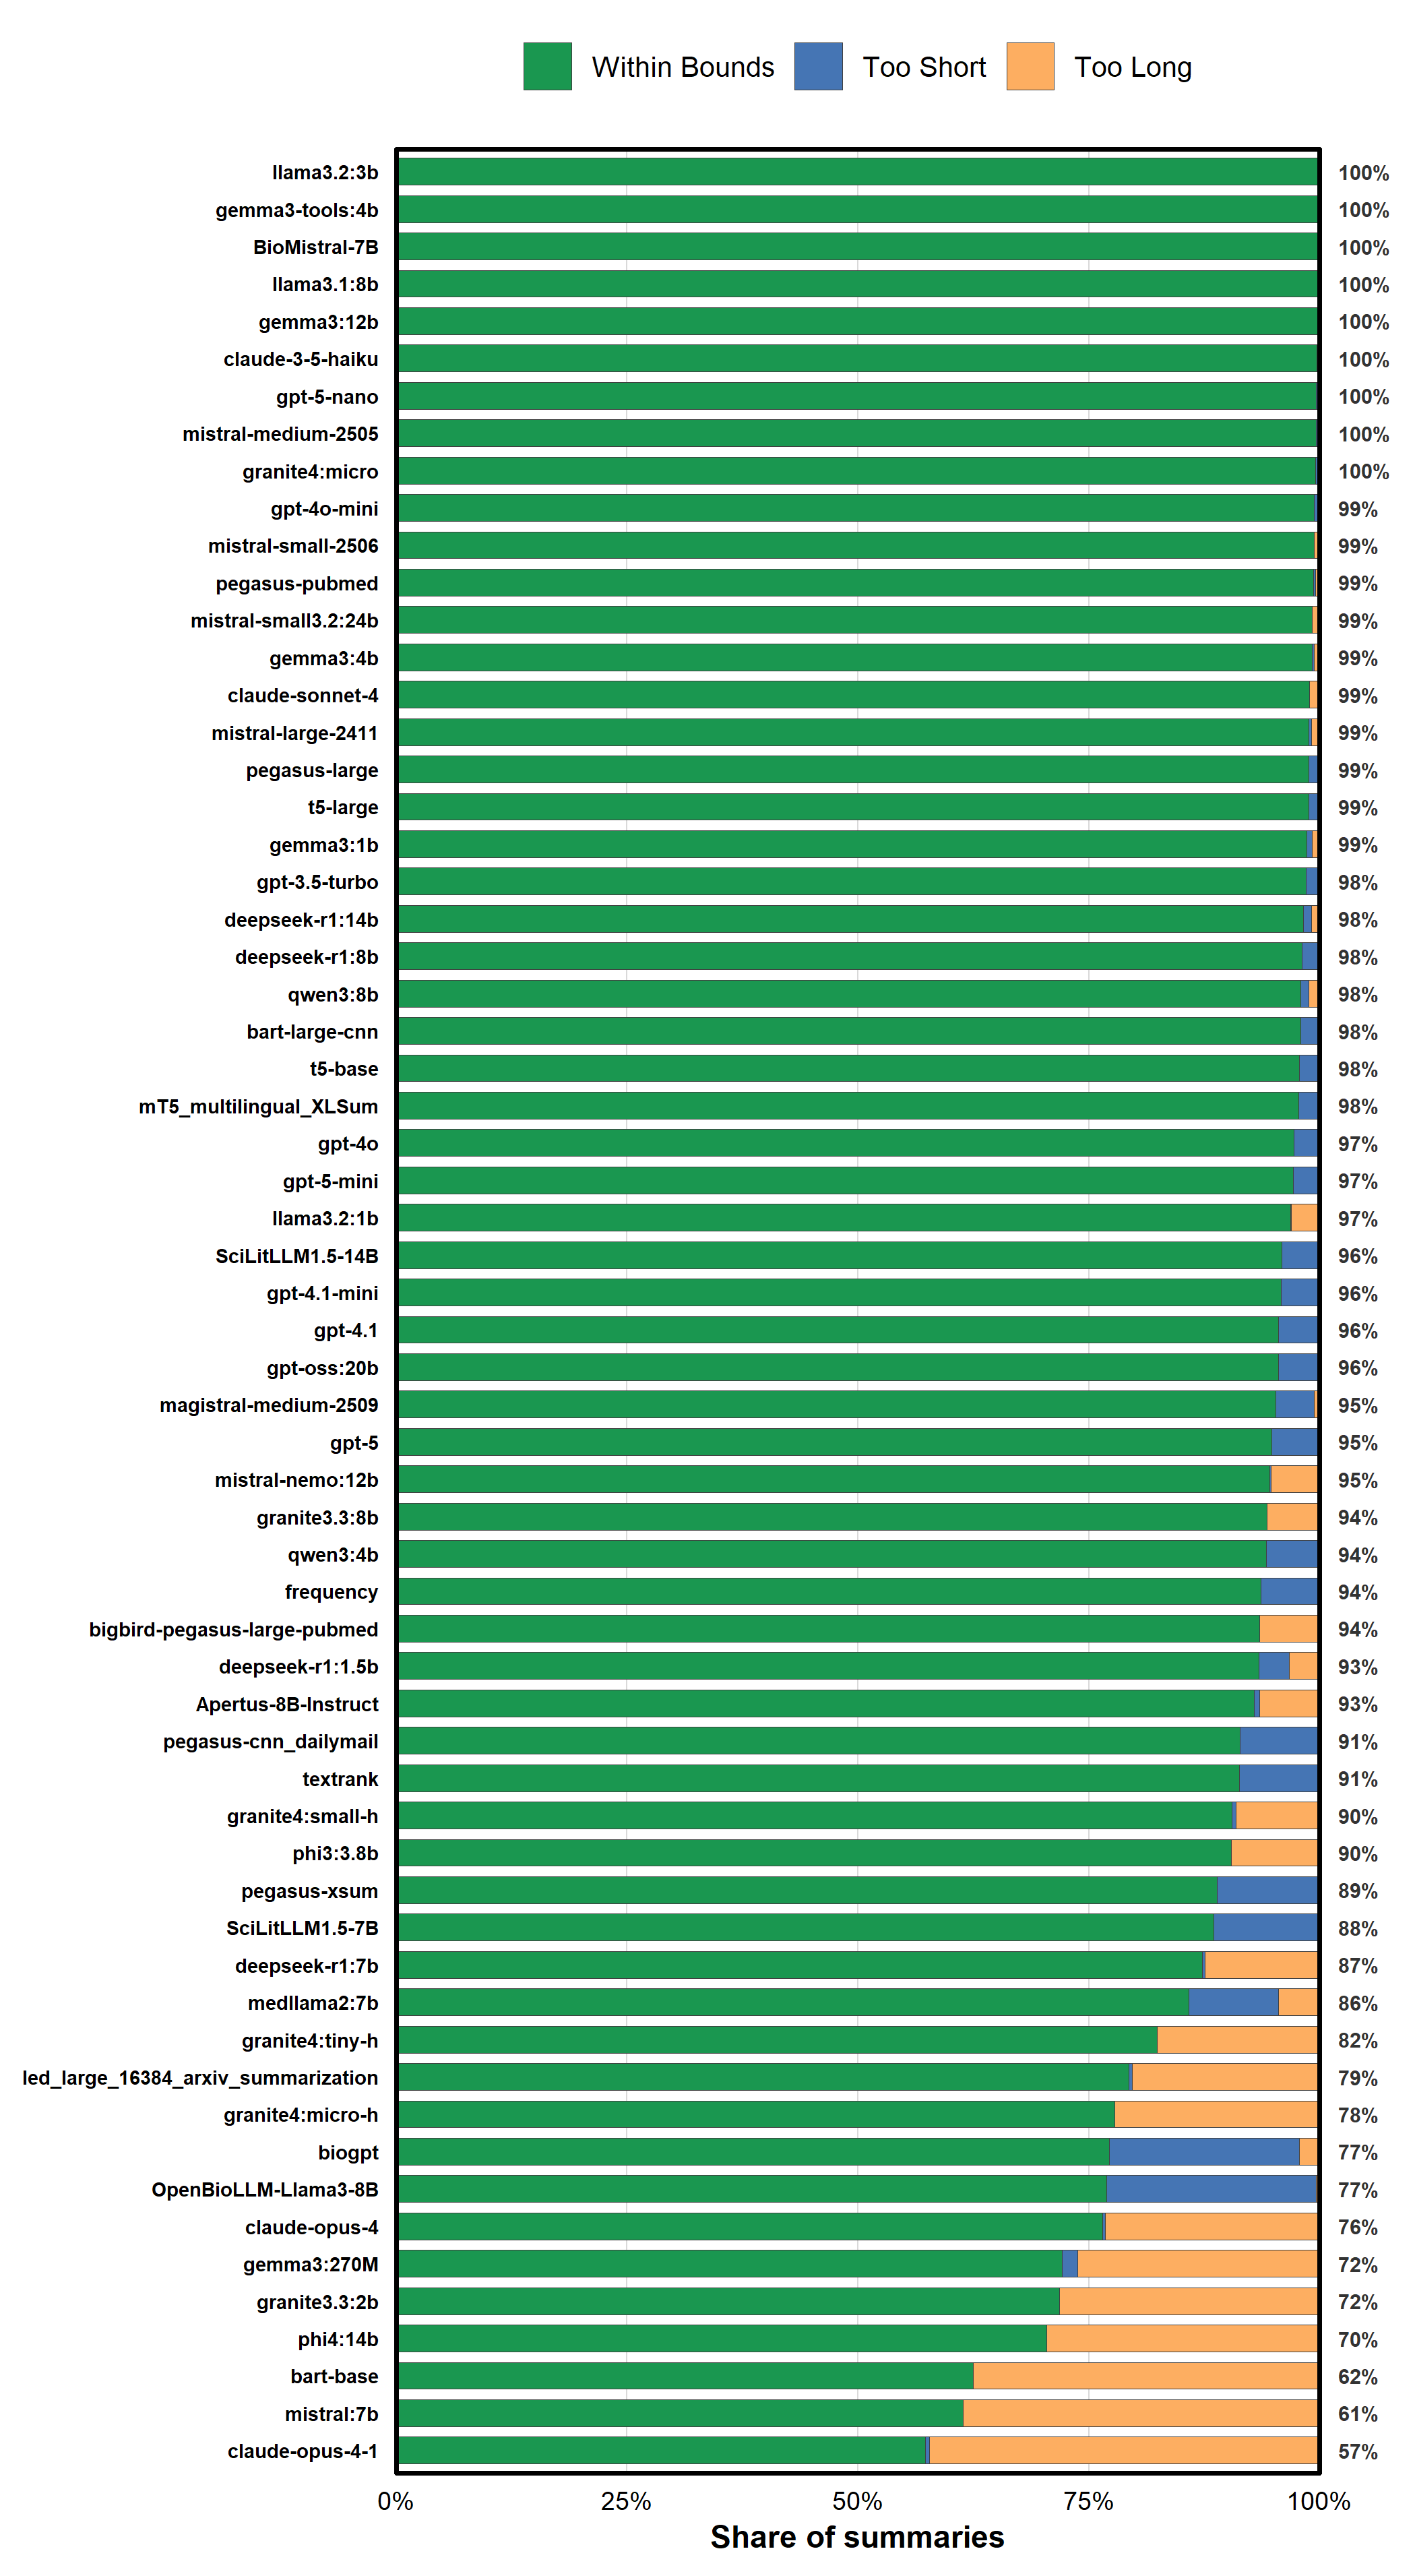
\includegraphics[height=0.75\textheight,keepaspectratio]{Visualizations/length_compliance.png}
    \caption{\textbf{Summary length compliance per method:} Proportion of generated summaries that fell within the target length of 15--100 words, were too short, or were too long, shown for each of the 62 evaluated methods. Methods are ordered by decreasing share of within-bounds summaries, with the within-bounds percentage annotated at the right of each bar.}
    \label{fig:length_compliance}
\end{figure}

\begin{figure}[H]
    \centering
    
\includegraphics[width=0.80\textwidth]{Visualizations/supplementary1.png}
    \caption{\textbf{Model performance across metrics:} Overview of the performance of all evaluated models across all metrics.}
    \label{fig:supplementary_overview}
\end{figure}

\clearpage
\begin{table*}[!htbp]
\centering
\scriptsize
\caption{\textbf{Training cutoff dates and potential overlap for all evaluated models:} 
The training cutoff indicates the latest point in time up to which a model may have been trained; the source of this information is given in a separate column (confirmed, community, estimated, or unknown). Potential overlap describes the percentage of benchmark articles published on or before the respective cutoff date and therefore represents the theoretical maximum share of articles that could have been present in the model's training data. Closed-source models are marked accordingly. Models are ordered by decreasing potential overlap.\label{tab:training_cutoff_overlap}}
\begin{tabularx}{\linewidth}{X l l r}
\toprule
\textbf{Model} & \textbf{Training cutoff} & \textbf{Source} & \textbf{Potential overlap (\%)} \\
\midrule
claude-sonnet-4-20250514 (closed-source) & 2025-03 & confirmed & 40.2 \\
claude-opus-4-20250514 (closed-source) & 2025-03 & confirmed & 40.2 \\
claude-opus-4-1-20250805 (closed-source) & 2025-03 & community & 40.2 \\
deepseek-r1:1.5b & 2025-01 & community & 33.1 \\
deepseek-r1:7b & 2025-01 & community & 33.1 \\
deepseek-r1:8b & 2025-01 & community & 33.1 \\
deepseek-r1:14b & 2025-01 & community & 33.1 \\
gpt-5-2025-08-07 (closed-source) & 2024-10 & community & 24.0 \\
gemma3:270M & 2024-08 & confirmed & 20.3 \\
gemma3:1b & 2024-08 & confirmed & 20.3 \\
gemma3:4b & 2024-08 & confirmed & 20.3 \\
gemma3:12b & 2024-08 & confirmed & 20.3 \\
PetrosStav/gemma3-tools:4b & 2024-08 & confirmed & 20.3 \\
phi4:14b & 2024-06 & confirmed & 13.8 \\
gpt-oss:20b & 2024-06 & community & 13.8 \\
gpt-4.1 (closed-source) & 2024-06 & confirmed & 13.8 \\
gpt-4.1-mini (closed-source) & 2024-06 & confirmed & 13.8 \\
gpt-5-nano-2025-08-07 (closed-source) & 2024-05 & community & 11.8 \\
gpt-5-mini-2025-08-07 (closed-source) & 2024-05 & community & 11.8 \\
granite3.3:2b & 2024-04 & estimated & 10.3 \\
granite3.3:8b & 2024-04 & estimated & 10.3 \\
claude-3-5-haiku-20241022 (closed-source) & 2024-04 & confirmed & 10.3 \\
swiss-ai/Apertus-8B-Instruct-2509 & 2024-03 & confirmed & 8.5 \\
Uni-SMART/SciLitLLM1.5-7B & 2024 & estimated & 6.6 \\
Uni-SMART/SciLitLLM1.5-14B & 2024 & estimated & 6.6 \\
facebook/bart-large-cnn & 2019 & estimated & 5.0 \\
facebook/bart-base & 2019 & estimated & 5.0 \\
google-t5/t5-base & 2019-04 & estimated & 5.0 \\
google-t5/t5-large & 2019-04 & estimated & 5.0 \\
csebuetnlp/mT5\_multilingual\_XLSum & 2020 & estimated & 5.0 \\
google/pegasus-xsum & 2020 & estimated & 5.0 \\
google/pegasus-large & 2020 & estimated & 5.0 \\
google/pegasus-cnn\_dailymail & 2020 & estimated & 5.0 \\
AlgorithmicResearchGroup/led\_large\_16384\_arxiv\_summarization & 2020 & estimated & 5.0 \\
google/pegasus-pubmed & 2020 & estimated & 5.0 \\
google/bigbird-pegasus-large-pubmed & 2020 & estimated & 5.0 \\
microsoft/biogpt & 2021 & estimated & 5.0 \\
aaditya/OpenBioLLM-Llama3-8B & 2023-03 & confirmed & 5.0 \\
BioMistral/BioMistral-7B & 2023 & estimated & 5.0 \\
llama3.1:8b & 2023-12 & confirmed & 5.0 \\
llama3.2:1b & 2023-12 & confirmed & 5.0 \\
llama3.2:3b & 2023-12 & confirmed & 5.0 \\
medllama2:7b & 2022-09 & confirmed & 5.0 \\
phi3:3.8b & 2023-10 & confirmed & 5.0 \\
gpt-3.5-turbo (closed-source) & 2021-09 & confirmed & 5.0 \\
gpt-4o (closed-source) & 2023-10 & confirmed & 5.0 \\
gpt-4o-mini (closed-source) & 2023-10 & confirmed & 5.0 \\
mistral:7b & --- & unknown & --- \\
mistral-nemo:12b & --- & unknown & --- \\
mistral-small3.2:24b & --- & unknown & --- \\
qwen3:4b & --- & unknown & --- \\
qwen3:8b & --- & unknown & --- \\
granite4:micro & --- & unknown & --- \\
granite4:micro-h & --- & unknown & --- \\
granite4:tiny-h & --- & unknown & --- \\
granite4:small-h & --- & unknown & --- \\
mistral-medium-2505 (closed-source) & --- & unknown & --- \\
magistral-medium-2509 (closed-source) & --- & unknown & --- \\
mistral-large-2411 (closed-source) & --- & unknown & --- \\
mistral-small-2506 (closed-source) & --- & unknown & --- \\
\bottomrule
\end{tabularx}
\end{table*}

\section*{Acknowledgments}

Enrico Bono is supported by a grant from the European Union's Horizon Europe Marie Skłodowska-Curie Actions Doctoral Networks program project PICKED (HORIZON--MSCA--2023--DN-01, grant number 101168626). 
Louiza Galou is supported by a grant from the European Union's Horizon Europe Marie Skłodowska-Curie Actions Doctoral Networks Industrial Doctorates program project PROMOTE (HORIZON--MSCA--2023--DN-01, grant number 101169245). 
Paul Perco and Matthias Ley are members of and would like to cordially thank the COST Action PerMediK, CA21165, supported by COST (European Cooperation in Science and Technology).
We gratefully acknowledge Dorota Wojenska for her support in optimizing the overview workflow figure (Figure~\ref{fig:workflow_graphic}).

\section*{Author contributions}

Conceptualization: M.L., P.P., E.B. and F.B.; 
Methodology: M.L., P.P., E.B. and F.B.; 
Software: M.L.; 
Formal analysis: F.B., E.B., P.P. and M.L.; 
Validation: E.B., F.B., L.F., P.P., M.L., L.G., K.K.-I., S.W., P.A. and K.K.; 
Writing---original draft: F.B., E.B., M.L. and P.P.; 
Writing---review \& editing: E.B., F.B., P.P., M.L., K.K., L.G., L.F., K.K.-I., P.A. and S.W.; 
Visualization: F.B. and E.B.; 
Supervision: M.L. and P.P.;
All authors have read and agreed to the published version of the manuscript.

\section*{Declaration of interests}

K.K. is co-founder and shareholder of Delta4 GmbH (Vienna, Austria). 
F.B., E.B., L.F., L.G., K.K.-I., S.W., P.A., P.P. and M.L. are employees of Delta4 GmbH (Vienna, Austria).

\section*{Declaration of generative AI and AI-assisted technologies in the writing process}

During the preparation of this work the author(s) used Anthropic (Claude Opus 4.5) and OpenAI (GPT-5) in order to enhance textual clarity and readability without introducing of new hypotheses or data. After using this tool/service, the author(s) reviewed and edited the content as needed and take(s) full responsibility for the content of the published article.

\bibliography{refs}

\end{document}
